% !TEX encoding = UTF-8
% !TEX TS-program = pdflatex
% !TEX root = ../tesi.tex

%**************************************************************
\chapter{Tecnologie}
\label{cap:tecnologie}
Questo capitolo ha l'obiettivo di presentare le tecnologie scelte per realizzare il sistema oltre a luogo e/o motivazioni che hanno portato a tali scelte.
%**************************************************************

%**************************************************************
\section{Prodotto}
    \subsection{AdonisJS}
    \label{tech:adonis}
    \textbf{AdonisJS} è il framework per Node.js scelto per la creazione della parte back-end.\\
    Nonostante la cosa non sia menzionata nel sito ufficiale, è evidente che l'ispirazione dei creatori di questo framework derivi da \textbf{Laravel} per \textbf{PHP} da cui Adonis riprende le logiche interne, architettura e sintassi trasportando il tutto a linguaggio \textbf{TypeScript}.

    \begin{figure}[h!]
        \centering
        
\includegraphics[width=5cm]{adonis-logo.png}
        \caption{Logo di \textbf{AdonisJS}}
    \end{figure}

    Il framework è stato consigliato (in modo non vincolante) da Sync Lab che ha esperienza in Laravel ed è interessata al suo studio per capirne il grado di maturità. Inoltre, non è richiesta l'architettura a microservizi il che rende Adonis una scelta coerente non supportandola out-of-the-box.
    \\\\
    Le feature di Adonis più rilevanti per questo progetto sono: gestione API REST, \textbf{middleware} [\autoref{impl:middleware}], \textbf{ORM Lucid} [\autoref{impl:orm}], autenticazione mediante \textbf{OAT} [\autoref{impl:oat}] e \textbf{Bouncer} [\autoref{impl:bouncer}].

    \subsection{CoinGecko-API}
    Libreria JavaScript per la comunicazione con \textbf{CoinGecko}.\\
    CoinGecko è un monitor di tassi di cambio delle crypto-valute che mette a disposizione una API REST gratuita fino a 50 richieste al secondo. Non è una libreria ufficiale ma è comunque raccomandata sul sito di CoinGecko.

    \begin{figure}[h!]
        \centering
        
\includegraphics[width=10cm]{coingecko-logo.png}
        \caption{Logo di \textbf{CoinGecko}}
    \end{figure}

    Nel back-end, viene utilizzata per il calcolo del rapporto ETH/\euro.
    Si è scelto di utilizzare questa libreria vista la sua semplicità.

    \subsection{web3.js}
    Popolare libreria JavaScript per la comunicazione con un nodo della rete Ethereum.

    \begin{figure}[h!]
        \centering
        
\includegraphics[width=5cm]{web3js-logo.jpg}
        \caption{Logo di \textbf{web3.js}}
    \end{figure}

    Nel back-end, viene utilizzata per la comunicazione con lo smart contract del token.

    \subsection{Infura}
    Node provider per connessione ad un nodo della blockchain Ethereum tramite protocollo \textbf{WebSocket} a cui web3.js si possa interfacciare.

    \begin{figure}[h!]
        \centering
        
\includegraphics[width=5cm]{infura-logo.png}
        \caption{Logo di \textbf{Infura}}
    \end{figure}

    Utilizzato perché:
    \begin{itemize}
        \item piano gratuito offre fino a 100.000 richieste al giorno, ottimo per testare un nuovo applicativo;
        \item non utilizzare un node provider vorrebbe dire creare un proprio nodo, cosa non fattibile dati gli ingenti requisiti a livello hardware per contenere ed elaborare l'intera blockchain.
    \end{itemize}

    \subsection{MariaDB}
    \label{tech:mariadb}
    Database relazionale basato su linguaggio \textbf{SQL} di dialetto \textbf{MySQL}.

    \begin{figure}[h!]
        \centering
        
\includegraphics[width=10cm]{mariadb-logo.png}
        \caption{Logo di \textbf{MariaDB}}
    \end{figure}

    Non c'erano particolari motivazioni che portassero alla scelta di un database relazionale specifico quindi questo è stato scelto per precedenti esperienze del programmatore.

%**************************************************************
\section{Ambiente di lavoro}
    \subsection{Kovan}
    Rete equivalente ad Ethereum mantenuta da un consorzio di sviluppatori Ethereum che viene utilizzata per fare test degli smart contract prima del loro (irreversibile) rilascio sulla \textit{main net} Ethereum. Il suo utilizzo è gratuito in quanto gli ETH validi solo per questa rete vengono concessi gratuitamente. Si basa sul \textbf{Proof-of-Authority} per il quale non vi è \textit{mining} ma i blocchi vengono inseriti da un'autorità centrale. Ciò rende le operazioni su Kovan più veloci e facilita il testing di nuovi smart contract.

    \begin{figure}[h!]
        \centering
        \includegraphics[width=6cm]{Kovan-logo.png}
        \caption{Logo di \textbf{Kovan}}
    \end{figure}

    Essendo questo un progetto didattico, lo smart contract di Sync Lab è stato rilasciato su rete Kovan.

    \subsection{Etherscan}
    Sito web che permette di monitorare wallet e smart contract di cui si conosca l'indirizzo e visualizzarne caratteristiche e transazioni in entrata/uscita.

    \begin{figure}[h!]
        \centering
        
\includegraphics[width=10cm]{etherscan-logo.png}
        \caption{Logo di \textbf{Etherscan}}
    \end{figure}

    Utilizzato per il debugging del back-end nelle sue interazioni con lo smart contract.

    \subsection{MetaMask}
    Plugin per browser \textbf{Chrome} e \textbf{Firefox} che permette la gestione dei propri wallet Ethereum, l'invio di ether e token ad altri wallet e l'interazione con gli smart contract integrati su front-end [\autoref{img:wallet}, \autoref{img:transaction}].

    \begin{figure}[h!]
        \centering
        
\includegraphics[width=10cm]{metamask-logo.png}
        \caption{Logo di \textbf{MetaMask}}
    \end{figure}

    Utilizzato per cambiare direttamente lo stato dello smart contract ed agevolare, dunque, il debugging del back-end nelle sue interazioni con esso.

    \subsection{Stoplight Studio}
    Applicazione a scopo documentale che consente di definire una API REST completa di definizione dei dati in input/output, status code e modalità di autorizzazione. Utilizzabile per testare l'API una volta completata.
    \\\\
    Utilizzato dal project manager per definire l'API che il back-end deve avere e con la quale il front-end deve interfacciarsi.

    \begin{figure}[h!]
        \centering
        \hspace*{-1cm}
        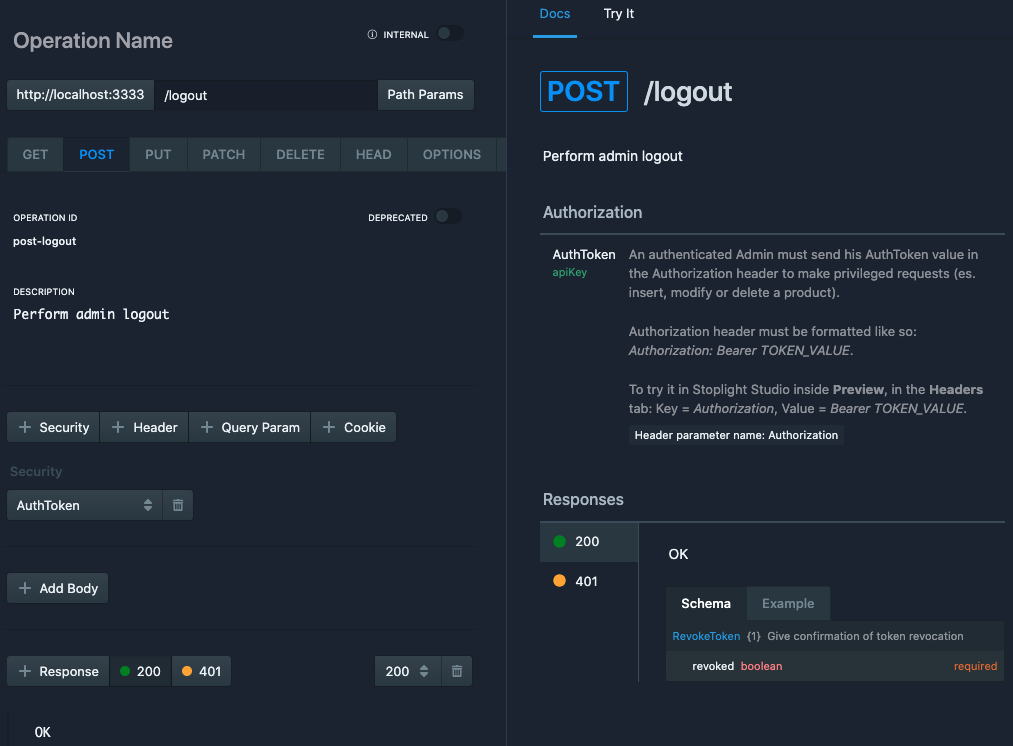
\includegraphics[width=16cm]{stoplight-screen.png}
        \caption{Schermata di \textbf{Stoplight Studio}}
    \end{figure}

\newpage

    \subsection{IntelliJ IDEA}
    \textbf{IDE} di \textbf{JetBrains} nato per la programmazione in Java.\\

    \begin{figure}[h!]
        \centering
        
\includegraphics[width=5cm]{intellij-logo.png}
        \caption{Logo di \textbf{IntelliJ IDEA}}
    \end{figure}

    Utilizzato come unico IDE del progetto in quanto nella sua vesione \textit{Ultimate} permette l'installazione di plugin che lo rendono equivalente ad altri IDE offerti da JetBrains come \textbf{WebStorm} per la programmazione in JavaScript/TypeScript e \textbf{DataGrip} per lo sviluppo in (e mantenimento di) database relazionali. Inoltre il plugin \textbf{Asciidoctor} è stato utilizzato per realizzare, nell'omonimo formato, il documento tecnico richiesto dall'azienda per questo prodotto.

    \subsection{Docker}
    Piattaforma per la creazione ed esecuzione di applicativi containerizzati (ovvero virtualizzati con virtualizzazione a livello di sistema operativo).

    \begin{figure}[h!]
        \centering
        
\includegraphics[width=6cm]{docker-logo.png}
        \caption{Logo di \textbf{Docker}}
    \end{figure}

    Utilizzato per creare l'ambiente di lavoro locale mettendo in piedi un'istanza di \textbf{MariaDB} [\autoref{tech:mariadb}] containerizzata che non richieda configurazione.

    \subsection{git}
    Sistema di versionamento distribuito creato da Linus Torvalds per il kernel Linux.

    \begin{figure}[h!]
        \centering
        
\includegraphics[width=5cm]{git-logo.png}
        \caption{Logo di \textbf{git}}
    \end{figure}

    Utilizzato come sistema di versionamento dell'applicativo per facilitare il lavoro concorrente con gli addetti al front-end.
